\documentclass[border=10pt]{standalone}

\usepackage{tikz}
\usepackage{tikzsymbols}
\usetikzlibrary{calc,patterns,shapes.geometric}

\def\centerarc[#1](#2)(#3:#4:#5){\draw[#1] ($(#2)+({#5*cos(#3)},{#5*sin(#3)})$) arc (#3:#4:#5);}

\begin{document}
	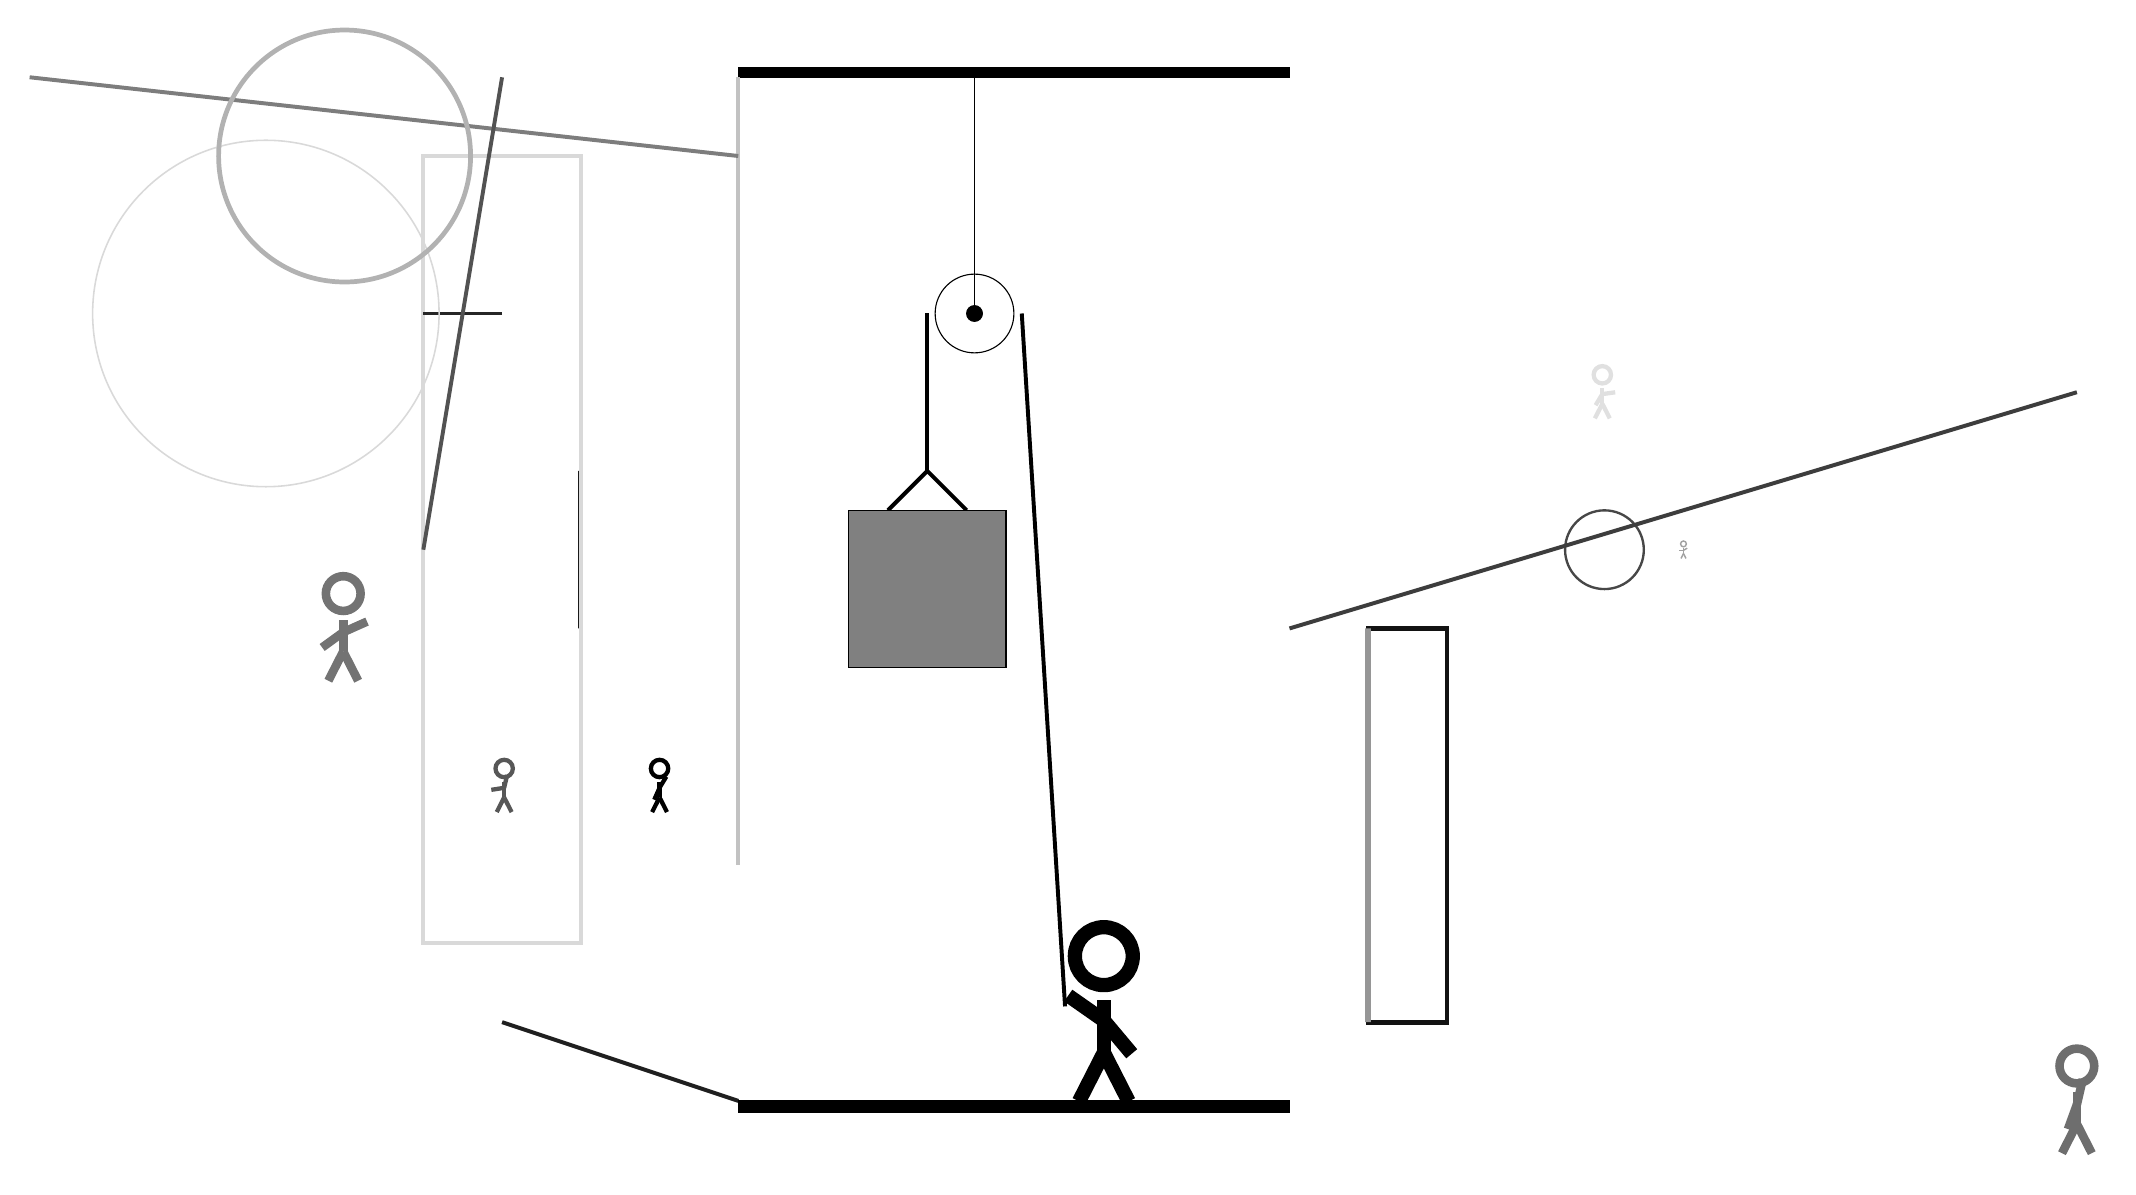
\begin{tikzpicture}
		%%%%% START %%%%%
		
		\draw[fill=black] (-2, 10) rectangle (5, 10.125);
		
		\draw (1, 7) circle (0.5);
		\draw[fill=black] (1, 7) circle (0.1);
		\draw (1, 10) -- (1, 7);
		
		\draw[line width=0.5mm] (-0.1, 4.5) -- (0.4, 5.0) -- (0.9, 4.5);
		\draw[fill=black!50] (-0.6, 4.5) rectangle (1.4, 2.5);
		
		\draw[line width=0.5mm] (0.4, 7) -- (0.4, 5.0);
		\centerarc[line width=0.5mm](1, 7)(0:180:0.6);
		\draw[line width=0.5mm](1.6, 7) -- (2.15, -1.8);
		
		\node at (2.6, -1.9) {\Strichmaxerl[10][-35][-50]};
		
		\draw[line width=0.6mm, color=black!90] (-4, 5) rectangle (-4, 3);
		
		\draw[line width=0.5mm, color=black!15] (-4, 9) rectangle (-6, -1);
		\draw[line width=0.6mm, color=black!93] (6, -2) rectangle (7, 3);
		\draw[line width=0.5mm, color=black!88](-5, -2) -- (-2, -3);
		\node[line width=0.3mm, color=black!12] at (9, 6) {\Strichmaxerl[3][59][8]};
		
		\draw [line width=0.3mm, color=black!72](9, 4) circle (0.5);
		
		\draw[line width=0.5mm, color=black!24](-2, 10) -- (-2, 0);
		\draw[line width=0.7mm, color=black!41] (6, 3) rectangle (6, -2);
		\node[line width=0.5mm, color=black!66] at (-5, 1) {\Strichmaxerl[3][9][77]};
		\node[line width=0.7mm, color=black!57] at (15, -3) {\Strichmaxerl[6][70][77]};
		\node[line width=0.7mm, color=black!55] at (-7, 3) {\Strichmaxerl[6][36][24]};
		
		\draw[line width=0.5mm, color=black!85](-5, 7) -- (-6, 7);
		\draw[line width=0.5mm, color=black!76](5, 3) -- (15, 6);
		
		\node[line width=0.6mm, color=black!37] at (10, 4) {\Strichmaxerl[1][0][30]};
		\node[line width=0.7mm, color=black!100] at (-3, 1) {\Strichmaxerl[3][66][59]};
		\draw[line width=0.5mm, color=black!51](-2, 9) -- (-11, 10);
		
		\draw [line width=0.2mm, color=black!15](-8, 7) circle (2.2);
		\draw [line width=0.6mm, color=black!30](-7, 9) circle (1.6);
		\draw[line width=0.5mm, color=black!68](-6, 4) -- (-5, 10);
		
		\draw[fill=black] (-2, -3) rectangle (5, -3.15);
		
		%%%%% END %%%%%
	\end{tikzpicture}
\end{document}